\chapter{Background}
\label{chap:Background}
This chapter will provide the reader with relevant information and background knowledge that are required to understand the proposed architecture. Indeed, the main concepts described hereunder are at the core of the employed methods and rationale behind the different intuitions. \\

To summarize, we will go through the main benefits of knowledge graphs and why they are gaining traction in the machine learning field. Then, the concept of Recurrent Neural Network (RNN) will be broached, a famous deep learning architecture to induce temporal correlation into a model. Finally, we will explore the concept and body of literature for evolving knowledge graphs and their applications.

\section{Knowledge Graphs}
\label{sec:Knowledge Graph}
Knowledge graphs model information through entities, properties of these entities and relationships between them. This kind of modelization of information allows to naturally combine different sources together and ultimately leverage information from data streams initially disparate. By managing to merge together these sources, the goal is to enrich our knowledge on the given entities and eventually leverage this additional linkage structure information with machine learning techniques. \\

\begin{wrapfigure}{r}{0.6\textwidth}
 \centering
 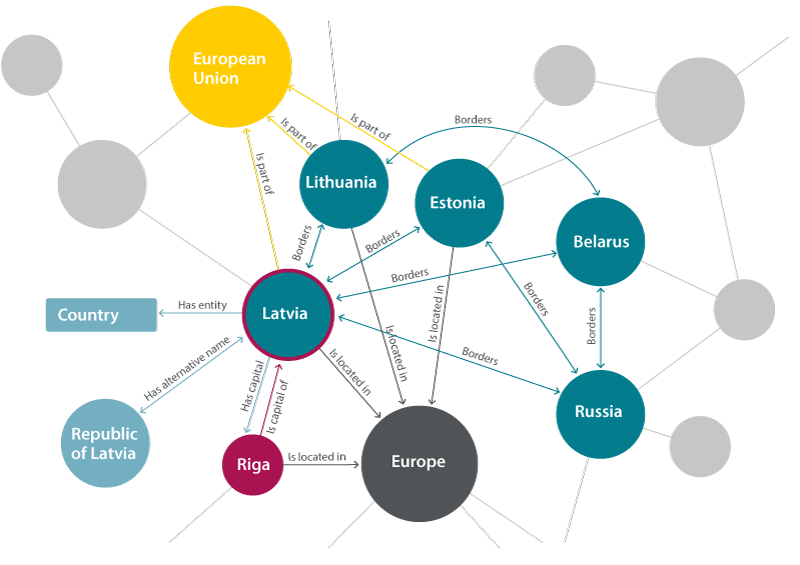
\includegraphics[width=.9\linewidth]{figures/kg-example.png}
 \captionsetup{width=.9\linewidth}
 \caption{An example of a knowledge graph representing how countries are related geographically.}
 \label{fig:kg-example}
\end{wrapfigure}

For example, on the figure~\ref{fig:kg-example}, we could imagine that geographical links (e.g. borders, is located in, \dots) come from a different source (e.g. OpenStreeMap) of information than the political links (e.g. is part of, has alternative name, \dots). In this enhanced graph combining information, two entities might be closer to each other (in terms of graph hops) than in any of the individual sources. \\

Finally, any algorithmic technique employed downstream could potentially make use of the edge type (e.g. borders, is part of, \dots) in the procedure, by giving more weights to specific edge types, for example. All in all, this allows for a much wider spread of potential techniques and information extraction algorithms or models. \\

For these reasons, representing and leveraging knowledge as such has a long history in machine learning and computer science as a whole~\cite{Minsky:1974:FRK:889222, Davis1993WhatIA}. In the last few years, this concept has gained a lot of traction in the scientific community as well as in the industry~\cite{LiuZhiyuan:247, 7358050} for obvious reasons. Indeed, the tremendous progress made in machine learning coupled with this idea of knowledge graph has been applied to many applications such as fraud detection (e.g. for a bank), community identification (e.g. in a social network), recommender systems (e.g. for an online shop). In such systems, it may be difficult for a human to make sense of the different links between entities and how their properties correlate as these links could be multiple hops away from each other. \\

In these previous examples, the entities, properties and relationships could be the following:
\paragraph{Bank knowledge graph: }
\begin{itemize}
 \item[] Entities and Properties:
 \begin{itemize}
  \item Person(First name, Last name, Address)
  \item Company(Name, Address)
  \item Account(Number, Type, Amount)
 \end{itemize}
 \item[] Relationships:
 \begin{itemize}
  \item Person -- \textit{is owner} -- Account
  \item Company -- \textit{is owner} -- Account
  \item Person -- \textit{work at} -- Company
  \item Account -- \textit{wire transfer} -- Account
 \end{itemize}
\end{itemize}
\paragraph{Social network knowledge graph: }
\begin{itemize}
 \item[] Entities and Properties:
 \begin{itemize}
  \item Person(First name, Last name)
  \item Group(Name)
  \item Content(Title)
 \end{itemize}
 \item[] Relationships:
 \begin{itemize}
  \item Person -- \textit{friend with} -- Person
  \item Person -- \textit{likes} -- Content
  \item Person -- \textit{belongs to} -- Group
 \end{itemize}
\end{itemize}
\paragraph{Online shop knowledge graph (figure~\ref{fig:kg-online-shop}): }
\begin{itemize}
 \item[] Entities and Properties:
 \begin{itemize}
  \item Client(First name, Last name)
  \item Category(Name)
  \item Product(Name, Price, Properties)
 \end{itemize}
 \item[] Relationships:
 \begin{itemize}
  \item Client -- \textit{purchased} -- Product
  \item Client -- \textit{follows} -- Category
  \item Product -- \textit{belongs to} -- Category
  \item Product -- \textit{shares property} -- Product
  \item Product -- \textit{has similar price} -- Product
 \end{itemize}
\end{itemize}

\newpage
\begin{figure}
	\centering
	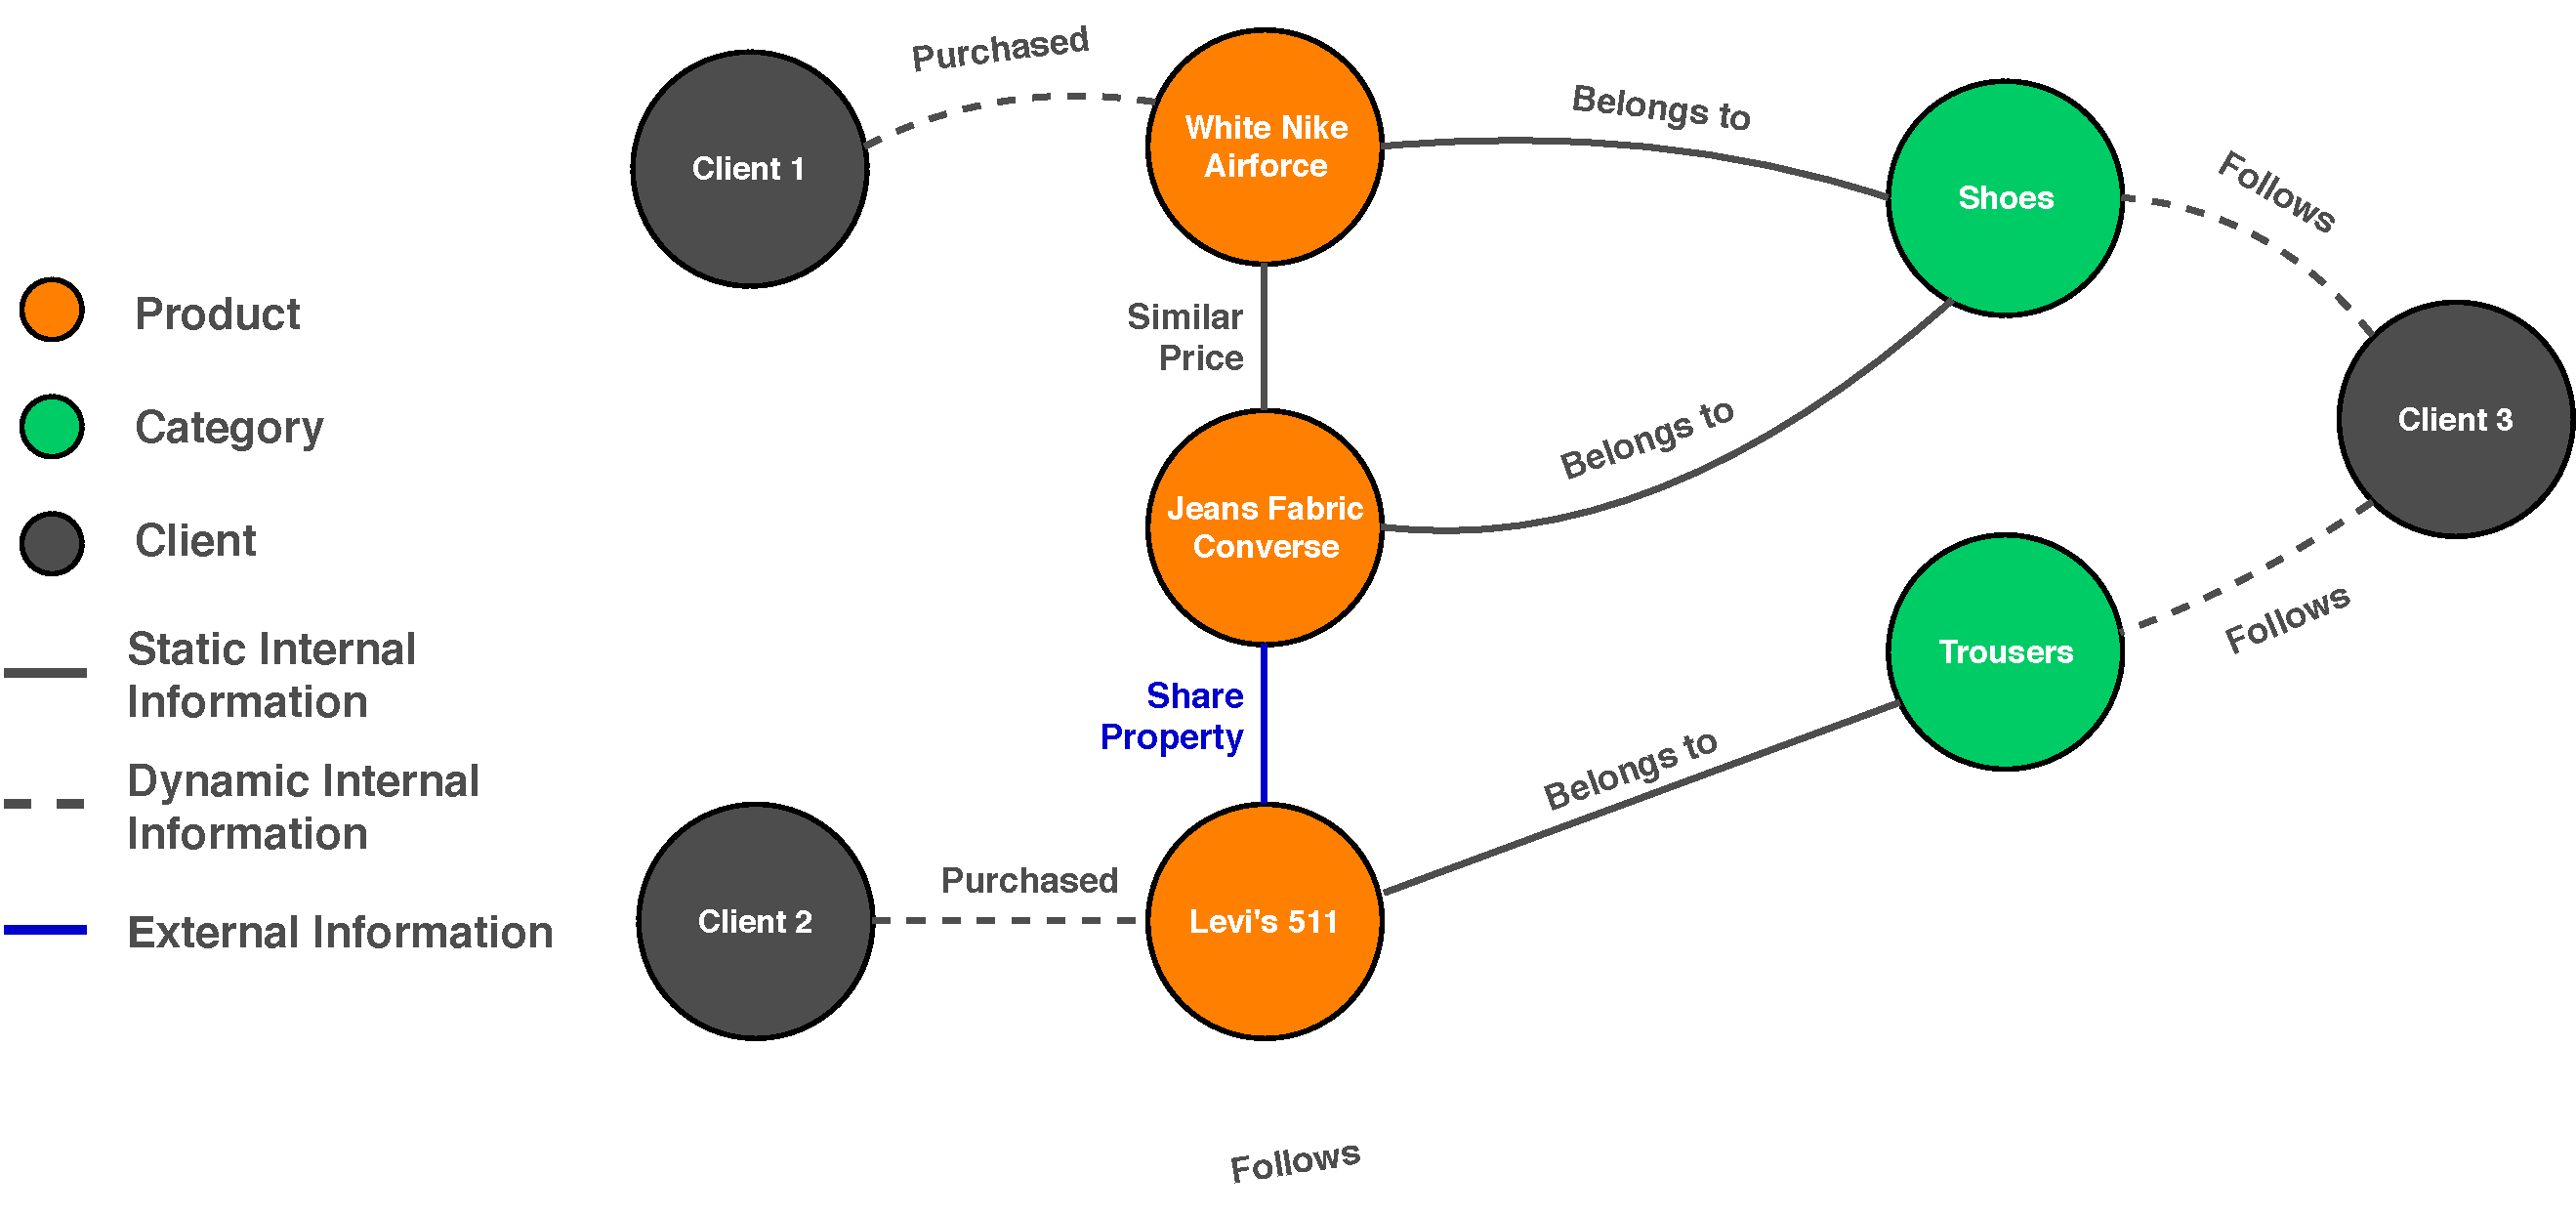
\includegraphics[width=.75\linewidth]{figures/kg-online-shop.pdf}
	\caption{
		An example of evolving knowledge graph for the ``Online Shop`` case described above. The evolution of the graph is shown through the labels $T=t$ for some edges. Indeed, the clients are buying, and generally performing actions, over time and the structure of the graph is evolving accordingly at different time step. The external information linking these \textit{Converse} shoes (made with jeans fabric) and a \textit{Levi's 511} may come from an external database to automatically map product identifiers to materials and fabrics they are made of.
	}
	\label{fig:kg-online-shop}
\end{figure}

\section{Recurrent Neural Network}
\label{sec:Recurrent Neural Network}
Recurrent Neural Network consists of a type of architecture for Deep Learning models that allows exploiting temporal dynamic behavior for sequence. This makes them particularly interesting and efficient for tasks that exhibit a temporal pattern, such as speech recognition or market forecasting. On top of that, this kind of architecture allows processing variable-length sequence input, which is not the case for most of the other machine learning (e.g. \textit{linear regression} or \textit{support vector machine}) or deep learning techniques (e.g. \textit{convolutional neural networks}).\\

Originally, these Recurrent Neural Networks were first heard of in 1986~\cite{10008954896} but the term \emph{recurrent} was not yet used to qualify the progress introduced in the paper. It is only three years later~\cite{6796948} that the term started to appear more actively in the research literature to qualify this type of neural networks. \\

At core of Recurrent Neural Networks, there are cells that rule how information is blended together from previous time steps and current step, and how much importance is given to these past and present steps. Technically, the RNN handles variable-length inputs by storing a hidden state that is recurrently updated at each time step based on its previous hidden state at time \emph{T-1}, and the current input at time \emph{T}. More formally, given a sequence of inputs $\bm{x} = (\bm{x}_1, \bm{x}_2, ..., \bm{x}_T)$, the hidden state $\bm{h}_t$ is updated following the equation:

\begin{equation}\label{eq:rnn_hidden}
\bm{h}_t = 
\begin{cases}
\bm{0}, & t=0 \\
f(\bm{h}_{t-1}, \bm{x}_t; \bm{\theta}), & \mbox{otherwise}
\end{cases}
\end{equation}

With \emph{f} refers to a non-linear function depending on some parameters $\bm{\theta}$. Typically, the equation~\ref{eq:rnn_hidden} is defined as:

\begin{equation}
 \bm{h}_t = f(U\bm{x}_t + W\bm{h}_{t-1} + \bm{b})
\end{equation}

Where the parameters $\bm{\theta}$ are the matrices \emph{W}, \emph{U} and the bias term $\bm{b}$, while the function \emph{f} is a smooth and bounded function such as sigmoid or a hyperbolic tangent. Finally, the sequence of outputs of the RNN $\bm{y} = (\bm{y}_1, \bm{y}_2, ..., \bm{y}_T)$ is usually defined as:

\begin{equation}
\bm{y}_t = g(V\bm{h}_t + \bm{c})
\end{equation}

Where the matrix \emph{V} and the bias vector $\bm{c}$ are learned parameters, while the function \emph{g} is often a \emph{softmax}. \\

Unfortunately, such networks are suffering from many problems while training to use \emph{back-propagation through time} or (\emph{BPTT}). Indeed, this architecture has difficulties capturing long-term dependencies in the input sequence because the gradient update has a tendency to take abnormally big values (i.e. explode) or small ones (i.e.e vanish, since they are squashed at every time steps by the bounded activation functions \emph{sigmoid} or \emph{tanh}). \\

To circumvent these two problems, researchers have designed more sophisticated activation functions, called cell in this case. The two principal types of cell are LSTM~\cite{doi:10.1162/neco.1997.9.8.1735} and GRU~\cite{DBLP:journals/corr/ChoMGBSB14}, the former predating the latter by almost 20 years. A schematic view of these types of cell can be found in~\ref{fig:cells} for a better understanding of the mechanisms ruling the learning dynamic. These are the typical go-to cells for any application requiring a Recurrent Neural Network. However there does not exist a rule of thumb to pick one of the two as this is usually dependent on the application and, more precisely, on the data at hand~\cite{DBLP:journals/corr/ChungGCB14}. Nonetheless, one interesting argument in favor of the GRU cell is that it depends on fewer parameters than LSTM, as they lack an output gate. It makes them particularly interesting when the computational resources are limited or when one wants to iterate over quick experiments. \\

\begin{figure}
 \centering
 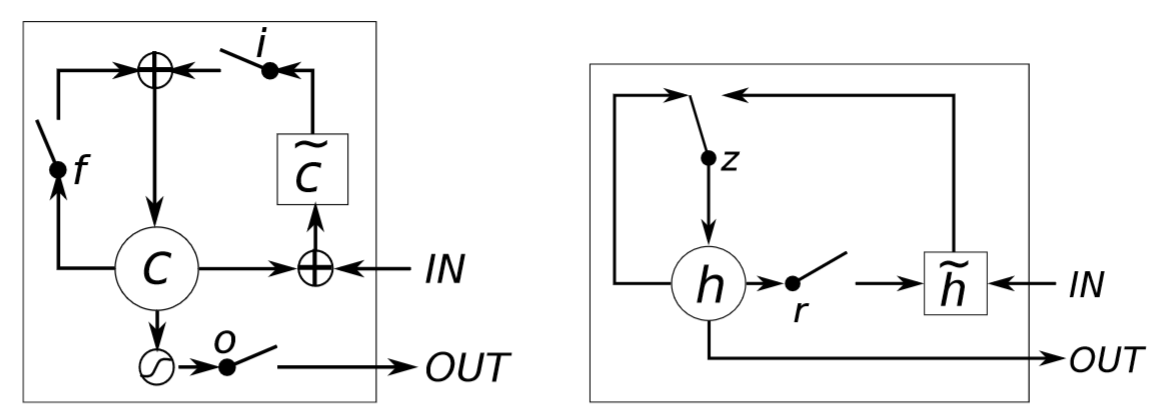
\includegraphics[width=.6\linewidth]{figures/rnn-cells.png}
 \captionsetup{width=.75\linewidth}
 \caption{
  The schematic views of an LSTM (\textit{left}) and GRU (\textit{right}) cell. On the left-hand cell, \emph{i}, \emph{o} and \emph{f} mean respectively \emph{input}, \emph{output} and \emph{forget} gates. Finally, on this same cell, \emph{c} and \emph{$\tilde{c}$} represents the old and new contents of the memory cell. For the right-hand cell, \emph{r} and \emph{z} are the reset and update gates while \emph{h} and \emph{$\tilde{h}$} are respectively the actual and new (or candidate) activation. Figure from~\cite{DBLP:journals/corr/ChungGCB14}.
 }
 \label{fig:cells}
\end{figure}

The equations defining the update dynamics of the hidden state, as well as the other parameters in these cells are the following:

\begin{multicols}{2}
 \centering
 \textbf{LSTM update equations}
 \begin{equation*}
  \begin{aligned}
   \bm{i}_t &= \sigma(U^i\bm{x}_t + W^i\bm{h}_{t-1}) \\
   \bm{f}_t &= \sigma(U^f\bm{x}_t + W^f\bm{h}_{t-1}) \\
   \bm{o}_t &= \sigma(U^o\bm{x}_t + W^o\bm{h}_{t-1}) \\
   \bm{\tilde{C}}_t &= tanh(U^g\bm{x}_t + W^g\bm{h}_{t-1}) \\
   \bm{C}_t &= \sigma(\bm{f}_t \odot \bm{x}_t + \bm{i}_t \odot \bm{\tilde{C}}_t) \\
   \bm{h}_t &= tanh(\bm{C}_t) \odot \bm{o}_t
  \end{aligned}
 \end{equation*}\columnbreak
 \vfill
 \textbf{GRU update equations}
 \begin{equation*}
  \begin{aligned}
   \bm{z}_t &= \sigma(U^z\bm{x}_t + W^z\bm{h}_{t-1}) \\
   \bm{r}_t &= \sigma(U^r\bm{x}_t + W^r\bm{h}_{t-1}) \\
   \bm{\tilde{h}}_t &= tanh(U^h\bm{x}_t + W^h(\bm{r}_t \odot \bm{h}_{t-1})) \\
   \bm{h}_t &= (1-\bm{z}_t) \odot \bm{h}_{t-1} + \bm{z}_t \odot \bm{\tilde{h}}_t
  \end{aligned}
 \end{equation*}
\end{multicols}

Finally, these two cells and all these equations are defining a \emph{causal} structure. That is, the output at time \emph{T} only depends and capture information from the past $1, ..., T-1$ through the learning dynamics. However, it may be interesting to have the output at each time step to \emph{depend on the whole sequence}, in applications where it makes sense. Indeed, if one is doing part-of-speech tagging, the tag of a given work not only depends on the preceding words but following ones. On the contrary, if one wants to run the model on an \textit{online} stream of data for example, it would be flawed to train the model with access to future time steps. \\

However, in many cases it is possible to train such models with information from previous and next states where the relevant architecture is called \emph{Bidirectional RNN}. This kind of model combines an RNN that moves forward and one that moves backward, to finally mix their respective output with a concatenation followed by a fully-connected layer. \\

To conduct our research, we picked GRU cells in our case for the reasons mentioned above, namely their efficiency that allows to iterate over different architectures and hyper-parameters faster. The use of bidirectional RNN or not will be a hyper-parameter tuned with the other ones.

\section{Evolving Knowledge Graph}
\label{sec:Evolving Knowledge Graph}
This last core concept tackles the problem of evolving knowledge graph, where the term \emph{evolving} refers to a dynamic component within the knowledge graph. Furthermore, it characterizes changes in the graphs that can be two fold: changes in the structure (e.g. new entities and links, such as a new \emph{company} in the ``Bank knowledge graph`` example in section~\ref{sec:Knowledge Graph}), changes in properties within entities (e.g. the \emph{product price} could evolve over time for the ``Online shop knowledge graph``). \\

Ultimately, the goal is to account for such dynamic behavior in the structure of the graph or its properties. Indeed, one could consider these changes as a sequence of graph states, each state representing the graph structure and property values at a given time \emph{T}. This additional information would benefit many applications and allow for much complex information interaction than a knowledge graph that remains static. However, incorporating temporal information into knowledge graph-based learning is still one of the major difficulties~\cite{LiuZhiyuan:247}. For this reason, a lot of efforts have been carried around the topic~\cite{D16-1260, 7527876, DBLP:journals/corr/TrivediDWS17, 8047276}, but there still remains a lot of challenges such as scalability to large real-world applications and capacity to capture dynamics in skewed graphs~\cite{DBLP:journals/corr/abs-1812-02289}. \\

With this in mind, we are seeking an architecture that is able to reason over time by capturing the different dynamics of the knowledge graph at the same time as leveraging its structure and relationships. 
